%% GENERATED by scripts/make_figure1.py -- edit the generator, not this file.
\documentclass[border=6pt]{standalone}
\usepackage{tikz}
\usetikzlibrary{arrows.meta}
\usepackage{sansmath}
\renewcommand{\familydefault}{\sfdefault}
\sansmath
\definecolor{ink}{HTML}{1B2430}
\definecolor{inkdim}{HTML}{5D7185}
\definecolor{gridc}{HTML}{C9D3DE}
\definecolor{sph}{HTML}{D9DEE4}
\definecolor{sub}{HTML}{C8CED6}
\definecolor{shellc}{HTML}{EEF1F5}
\definecolor{uhi}{HTML}{1D3A7A}
\definecolor{ulo}{HTML}{F5DFA0}
\definecolor{spA}{HTML}{1D3A7A}
\definecolor{spB}{HTML}{A4C639}
\definecolor{spAB}{HTML}{2BB3A3}
\tikzset{
  gridl/.style={draw=gridc, line width=0.5pt},
  gridb/.style={draw=gridc!70!ink, line width=0.6pt},
  shell/.style={fill=shellc},
  op/.style={-{Stealth[length=7pt,width=5pt]}, line width=1.4pt, ink},
  mv/.style={-{Stealth[length=4pt,width=3.5pt]}, line width=0.9pt, ink},
  gen/.style={-{Stealth[length=5pt]}, line width=0.9pt, inkdim},
  lbl/.style={font=\small, ink},
  reads/.style={-{Stealth[length=5pt]}, line width=0.9pt, inkdim, dashed},
}
\newcommand{\num}[1]{\tikz[baseline=(n.base)]\node[draw=ink, circle, line width=0.6pt, inner sep=0.8pt, font=\scriptsize](n){#1};}
\begin{document}
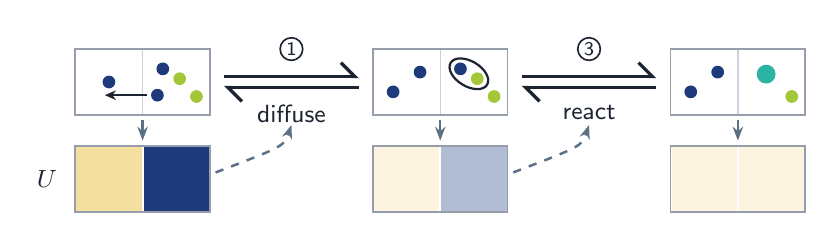
\begin{tikzpicture}[x=0.9cm, y=0.88cm]
\draw[gridl, shift={(3.100,-1.150)}] (0,0) grid[step=0.950] (1.900,0.950);
\draw[gridb] (3.100,-1.150) rectangle (5.000,-0.200);
\fill[spA] (3.575,-0.675) circle (2.3pt);
\fill[spA] (4.259,-0.865) circle (2.3pt);
\fill[spA] (4.335,-0.485) circle (2.3pt);
\fill[spB] (4.573,-0.627) circle (2.3pt);
\fill[spB] (4.810,-0.884) circle (2.3pt);
\draw[gen] (4.050,-1.230) -- (4.050,-1.520);
\draw[gridl, shift={(7.300,-1.150)}] (0,0) grid[step=0.950] (1.900,0.950);
\draw[gridb] (7.300,-1.150) rectangle (9.200,-0.200);
\fill[spA] (7.585,-0.817) circle (2.3pt);
\fill[spA] (7.965,-0.532) circle (2.3pt);
\fill[spA] (8.535,-0.485) circle (2.3pt);
\fill[spB] (8.772,-0.627) circle (2.3pt);
\fill[spB] (9.010,-0.884) circle (2.3pt);
\draw[gen] (8.250,-1.230) -- (8.250,-1.520);
\draw[gridl, shift={(11.500,-1.150)}] (0,0) grid[step=0.950] (1.900,0.950);
\draw[gridb] (11.500,-1.150) rectangle (13.400,-0.200);
\fill[spA] (11.785,-0.817) circle (2.3pt);
\fill[spA] (12.165,-0.532) circle (2.3pt);
\fill[spAB] (12.849,-0.561) circle (3.4pt);
\fill[spB] (13.210,-0.884) circle (2.3pt);
\draw[gen] (12.450,-1.230) -- (12.450,-1.520);
\draw[mv] (4.107,-0.865) -- ++(-0.589,0.000);
\draw[ink, line width=0.8pt, rotate around={-31.0:(8.654,-0.556)}] (8.654,-0.556) ellipse (0.300 and 0.181);
\draw[-{Straight Barb[left,length=5pt]}, line width=1.2pt, ink] (5.200,-0.595) -- (7.100,-0.595);
\draw[-{Straight Barb[left,length=5pt]}, line width=1.2pt, ink] (7.100,-0.755) -- (5.200,-0.755);
\node[lbl, above=4pt] at (6.150,-0.675) {\num{1}};
\node[lbl, below=5pt] at (6.150,-0.675) {diffuse};
\draw[-{Straight Barb[left,length=5pt]}, line width=1.2pt, ink] (9.400,-0.595) -- (11.300,-0.595);
\draw[-{Straight Barb[left,length=5pt]}, line width=1.2pt, ink] (11.300,-0.755) -- (9.400,-0.755);
\node[lbl, above=4pt] at (10.350,-0.675) {\num{3}};
\node[lbl, below=5pt] at (10.350,-0.675) {react};
\draw[reads] (5.080,-1.980) .. controls (6.050,-1.600) .. (6.150,-1.295);
\draw[reads] (9.280,-1.980) .. controls (10.250,-1.600) .. (10.350,-1.295);
\node[lbl, anchor=east] at (2.980,-2.075) {$U$};
\fill[ulo!100!white] (3.100,-2.550) rectangle ++(0.950,0.950);
\fill[uhi!100!white] (4.050,-2.550) rectangle ++(0.950,0.950);
\draw[white, line width=0.7pt, shift={(3.100,-2.550)}] (0,0) grid[step=0.950] (1.900,0.950);
\draw[gridb] (3.100,-2.550) rectangle (5.000,-1.600);
\fill[ulo!34!white] (7.300,-2.550) rectangle ++(0.950,0.950);
\fill[uhi!34!white] (8.250,-2.550) rectangle ++(0.950,0.950);
\draw[white, line width=0.7pt, shift={(7.300,-2.550)}] (0,0) grid[step=0.950] (1.900,0.950);
\draw[gridb] (7.300,-2.550) rectangle (9.200,-1.600);
\fill[ulo!34!white] (11.500,-2.550) rectangle ++(0.950,0.950);
\fill[ulo!34!white] (12.450,-2.550) rectangle ++(0.950,0.950);
\draw[white, line width=0.7pt, shift={(11.500,-2.550)}] (0,0) grid[step=0.950] (1.900,0.950);
\draw[gridb] (11.500,-2.550) rectangle (13.400,-1.600);
\end{tikzpicture}
\end{document}
